% !TeX encoding = UTF-8
%% Простая презентация с примером включения программного кода и
%% пошаговых спецэффектов
\documentclass[10pt]{beamer}
\usetheme{SPbAU}
%\useoutertheme{infolines}
\usepackage{fontspec}
\usepackage{xunicode}
\usepackage{xltxtra}
\usepackage{xecyr}
\usepackage{hyperref}
%% Minted для подсветки кода
\usepackage{minted}
\usepackage{listings}

\setminted[kotlin]{xleftmargin=\parindent, linenos, autogobble, frame=lines, escapeinside=\#\#}
\setminted[text]{xleftmargin=\parindent, autogobble, frame=lines, escapeinside=\#\#}

\usepackage{setspace}

\setmainfont[Mapping=tex-text]{DejaVu Serif}
\setsansfont[Mapping=tex-text]{DejaVu Sans}
\setmonofont[Mapping=tex-text]{DejaVu Sans Mono}
\usepackage{polyglossia}
\setdefaultlanguage{russian}
\usepackage{graphicx}
\usepackage{listings}
\lstdefinestyle{mycode}{
  belowcaptionskip=1\baselineskip,
  breaklines=true,
  xleftmargin=\parindent,
  showstringspaces=false,
  basicstyle=\footnotesize\ttfamily,
  keywordstyle=\bfseries,
  commentstyle=\itshape\color{gray!40!black},
  stringstyle=\color{red},
  numbers=left,
  numbersep=5pt,
  numberstyle=\tiny\color{gray},
}
\lstset{escapechar=@,style=mycode}

\newcommand{\code}[1]{\texttt{#1}}

\graphicspath{{img/}}

\definecolor{schema-keyword}{RGB}{0, 0, 128}
\newcommand{\keyword}[1]{\textbf{\textcolor{schema-keyword}{#1}}}
\usepackage[style=verbose,backend=biber]{biblatex}
\addbibresource{pres.bib}

\renewbibmacro*{in:}{%
	\iffieldundef{year}
	{}
	{\printtext{\bibstring{in}\intitlepunct}}}



\begin{document}
\title[Поиск списываний в контестах]{Поиск списываний в контестах по программированию с помощью построения графов зависимостей программ}

\author[Анисимова К.В.]{Анисимова Карина Витальевна\\{\footnotesize\textcolor{gray}{научный руководитель: А.В. Садовников}}}
\institute{НИУ ВШЭ - Санкт-Петербург}
\date{19 января 2022 г.}
\frame{\titlepage}

\begin{frame}[fragile]\frametitle{Введение в область}
	\begin{itemize}
		\item Число контестов, проводимых онлайн, растет
		\item Число нечестных участников растет
		\item Списывания практически не отслеживаются
		\item Необходимо большое количество сравнений
		\item Специфические модификации
	\end{itemize}
\end{frame}

\begin{frame}\frametitle{Задача поиска списывания}
		\hspace{-0.5cm}
Основные модификации\footnote[frame]{GPLAG: Detection of Software Plagiarism by Program Dependence Graph Analysis (2006)}\footnote[frame]{Finding Plagiarisms among a Set of Programs with JPlag(2003)}\footnote[frame]{Comparison and evaluation of code clone detection techniques and tools: A qualitative approach (2009)}:
\begin{columns}
  \column{0.5\textwidth}
  \centering
  \includegraphics[scale=0.7]{clear.png}
  
  \column{0.5\textwidth}
  \centering
  \begin{itemize}
  	\item Добавление/удаление комментариев
  	\item Добавление незначимых строк кода
  	\item Переименование
  	\item Перестановка операций
  	\item Взаимозаменяемые конструкции
  	\begin{itemize}
  		\item for/while
  		\item if/else
  	\end{itemize}
  \end{itemize}
\end{columns}
\end{frame}

\begin{frame}[fragile]\frametitle{Задача поиска списывания}
	\begin{columns}[T]
		\column{0.5\textwidth}
		\centering
		\includegraphics[scale=0.7]{comment.png}
		
		\column{0.5\textwidth}
		\centering
		\begin{itemize}
			\item Добавление/удаление комментариев
			\textcolor{gray}{
				\item Добавление незначимых строк кода
			\item Переименование
			\item Перестановка операций
			\item Взаимозаменяемые конструкции
		}
			\begin{itemize}
				\item \textcolor{gray}{for/while
				\item if/else
			}
			\end{itemize}
		\end{itemize}
	\end{columns}
\end{frame}

\begin{frame}[fragile]\frametitle{Задача поиска списывания}
	\begin{columns}[T]
		\column{0.5\textwidth}
		\centering
		\includegraphics[scale=0.7]{insert.png}
		
		\column{0.5\textwidth}
		\centering
		\begin{itemize}
			\item \textcolor{gray}{Добавление/удаление комментариев}
				\item Добавление незначимых строк кода
				\textcolor{gray}{
				\item Переименование
				\item Перестановка операций
				\item Взаимозаменяемые конструкции
			}
			\begin{itemize}
				\item \textcolor{gray}{for/while
					\item if/else
				}
			\end{itemize}
		\end{itemize}
	\end{columns}
\end{frame}

\begin{frame}[fragile]\frametitle{Задача поиска списывания}
	\begin{columns}[T]
		\column{0.5\textwidth}
		\centering
		\includegraphics[scale=0.7]{renamed.png}
		
		\column{0.5\textwidth}
		\centering
		\begin{itemize}
			\item \textcolor{gray}{Добавление/удаление комментариев
			\item Добавление незначимых строк кода}
				\item Переименование
				\textcolor{gray}{
				\item Перестановка операций
				\item Взаимозаменяемые конструкции
			}
			\begin{itemize}
				\item \textcolor{gray}{for/while
					\item if/else
				}
			\end{itemize}
		\end{itemize}
	\end{columns}
\end{frame}

\begin{frame}[fragile]\frametitle{Задача поиска списывания}
	\begin{columns}[T]
		\column{0.5\textwidth}
		\centering
		\includegraphics[scale=0.7]{reordering.png}
		
		\column{0.5\textwidth}
		\centering
		\begin{itemize}
			\item \textcolor{gray}{Добавление/удаление комментариев
				\item Добавление незначимых строк кода
			\item Переименование}
				\item Перестановка операций
				\textcolor{gray}{
				\item Взаимозаменяемые конструкции
			}
			\begin{itemize}
				\item \textcolor{gray}{for/while
					\item if/else
				}
			\end{itemize}
		\end{itemize}
	\end{columns}
\end{frame}

\begin{frame}[fragile]\frametitle{Задача поиска списывания}
	\begin{columns}[T]
		\column{0.5\textwidth}
		\centering
		\includegraphics[scale=0.7]{control.png}
		
		\column{0.5\textwidth}
		\centering
		\begin{itemize}
			\item \textcolor{gray}{Добавление/удаление комментариев
				\item Добавление незначимых строк кода
				\item Переименование
			\item Перестановка операций}
				\item Взаимозаменяемые конструкции
			\begin{itemize}
				\item for/while
					\item if/else
			\end{itemize}
		\end{itemize}
	\end{columns}
\end{frame}

\begin{frame}\frametitle{Program Dependency Graph}
	\begin{columns}
		\column{0.6\textwidth}
		\begin{definition}
			\textbf{Program Dependency Graph (PDG)} -- представление программы в виде графа. \\
			\textbf{Вершинами} являются базовые выражения. \\
			\textbf{Ребра зависимости по данным} соединяют вершины, в которых используются одинаковые данные. \\
			\textbf{Ребра передачи управления} соединяют две вершины, если контролирующая вершина определяет, будет ли выполняться выражение в зависимой вершине.
		\end{definition}
		
		\column{0.51\textwidth}
		\flushleft \hspace*{0.6cm}\includegraphics[scale=0.65]{pdg_code.png}
		\includegraphics[scale=0.28]{pdg_example.png}
		\newline
		
	\end{columns}
\end{frame}


\begin{frame}[fragile]\frametitle{Существующие решения и аналоги}
	\begin{itemize}
		\item Антиплагиат
		\begin{itemize}
			\item проверяет код как обычный текст
		\end{itemize}
		\item SIM \footnote[frame]{Sim: A Utility For Detecting Similarity in Computer Programs (1999)}
		\begin{itemize}
			\item справляется с форматированием и переименованием
			\item С, Java, Pascal
		\end{itemize}
	    \item Moss \footnote[frame]{MOSS, A System for Detecting Software Plagiarism(2002)}
	    \begin{itemize}
	    	\item справляется с форматированием и переименованием
	    	\item С/C++, C#, Java, assembly
	    \end{itemize}
		\item GPLAG \footnote[frame]{GPLAG: Detection of Software Plagiarism by Program Dependence Graph Analysis (2006)}
		\begin{itemize}
			\item Справляется со всеми основными модификациями
			\item Только для Java
			\item Оценка качества поиска контестного плагиата не проводилась
			\item Код утерян
		\end{itemize}
	\end{itemize}
\end{frame}

\begin{frame}\frametitle{Постановка цели и задачи}
    \textbf{Цель:} Оценить применимость алгоритма GPLAG к решению задачи поиска контестного плагиата
    
    \textbf{Задачи:}
    \begin{itemize}
        \item Реализовать алгоритм GPLAG, так как работающей версии не существует
        \item Собрать датасет для оценки применимость подхода
        \item Провести тестирование и проанализировать работу полученного решения
    \end{itemize}
\end{frame}

\begin{frame}\frametitle{Алгоритм}
	\begin{columns}
		\column{0.6\textwidth}
		\hspace*{-0.6cm}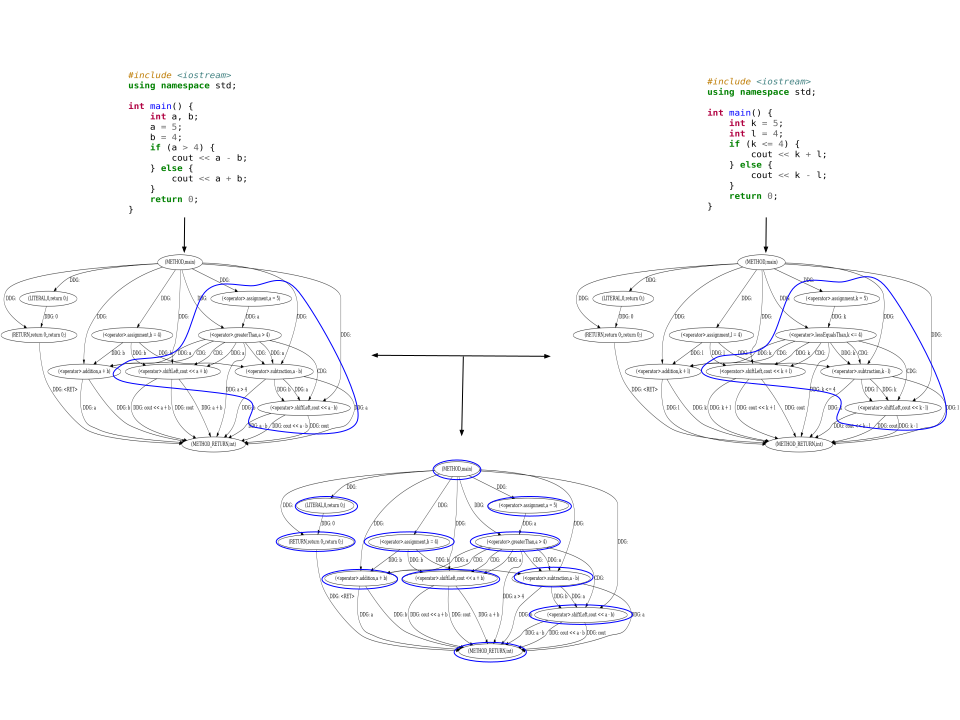
\includegraphics[scale=0.6]{algo.png}
		\column{0.4\textwidth}
		\centering
		\begin{enumerate}
			\item Построение PDG с помощью Joern
			\newline
			\item Сравнение графов
			\newline
			\newline
			\item Оценка покрытия графа
		\end{enumerate}
	\end{columns}
\end{frame}
    
\begin{frame}\frametitle{Реализация алгоритма. Сравнение графов}
	\begin{columns}[T]
	\column{0.5\textwidth}
	    Проблемы:
		\begin{enumerate}
		\item Алгоритмы поиска изоморфизмов вида граф - подграф не
		подходят
		\item Подграфов в графах слишком много
		\item Нужно учитывать типы вершин и ребер
		\end{enumerate}
	
	\column{.02\textwidth}
	
	\column{0.5\textwidth}
	Решения:
	\begin{enumerate}
	\item Сводим задачу к поиску изоморфизмов граф - подграф \newline
	\item Фиксируем размер подграфов: 9 вершин.
	\item Сужаем типы вершин до 60 основных
	\end{enumerate}
	\end{columns}
 
\end{frame}

\begin{frame}\frametitle{Построение датасета}
	Общедоступного датасета нет, поэтому необходимо его собрать.
	\newline
	\newline
	Датасет для оценки способности алгоритма находить плагиат и чувствительности к разным видам модификаций:
	\begin{itemize}
		\item 372 программы из 23 контестов с Codeforces
		\item С помощью инструмента gorshochek построены модификации:
		\begin{itemize} 
			\item Добавление/удаление комментариев
			\item Переименование
			\item Замена взаимозаменяемыех конструкций
		\end{itemize}
		\item Добавлена возможность построения модификации вставки незначимых строк кода в gorshochek
		\item Для каждой программы построен файл с случайным набором модификаций
	\end{itemize}
	
\end{frame}

\begin{frame}\frametitle{Построение датасета}
	Датасет для оценки работы алгоритма в случаях отсутствия плагиата:
	\begin{itemize}
		\item 23 программы, решающих одну и ту же простую задачу
		\item 12 программ, решающих одну и ту же сложную задачу
	\end{itemize}
	
\end{frame}

\begin{frame}\frametitle{Тестирование. Детали}
	\begin{itemize}
		\item Похожесть = $\frac{\text{Полученное покрытие}}{\text{Максимальное покрытие}}$
		\item При сравнении графов получаем покрытие
		\item Максимальное покрытие - покрытие полученное при сравнении программы с собой
	\end{itemize}
    
\end{frame}

\begin{frame}\frametitle{Тестирование. Результаты}
	\hspace*{-0.6cm}
	\includegraphics[scale=0.6]{res0.png}
	\hspace*{-0.6cm}
	Вывод: в случае наличия плагиата алгоритм показывает \hspace*{-0.6cm} достаточно большое значение похожести
	
	
	\hspace*{-0.6cm}
	\includegraphics[scale=0.6]{res1.png}
	\hspace*{-0.6cm}
	Вывод: в случае отсутствия плагиата алгоритм показывает \hspace*{-0.6cm} достаточно маленькое значение похожести, но в случаях \hspace*{-0.6cm} маленьких программ результат неоднозначный
	
\end{frame}


\begin{frame}\frametitle{Итоги}
	\begin{itemize}
		\item Реализован алгоритм из статьи GPLAG, поддержана гибкость в работе с разными языками программирования и разными подходами к построению PDG
		\item Собран датасет из 1895 программ для оценки возможности применения алгоритма к поиску контестного плагиата
		\item Проведено исследование и доказана применимость алгоритма GPLAG
		\newline
	\end{itemize}

    Репозиторий: \href{https://github.com/Karina5005/Plagiarism}{github.com/Karina5005/Plagiarism}
\end{frame}

\begin{frame}\frametitle{Дальнейшие планы}
    \begin{itemize}
    	\item Оценить точность других алгоритмов поиска плагата в применении к задаче поиска списываний в контестах
        \item Заменить в системе построение PDG по абстрактному синтаксису на построение PDG по assembler и сравнить эти два подхода
        \item Придумать и применить эвристики для ускорения поиска подграфов и сокращения их количества без сильной потери точности работы алгоритма
        \item Решить проблему нахождения плагиата в случаях популярных паттернов
        
    \end{itemize}
\end{frame}

\begin{frame}\frametitle{Тестирование. Результаты}
	\begin{columns}
		\column{0.5\textwidth}
		\centering
		\includegraphics[scale=0.52]{res.png}
		
		\column{0.5\textwidth}
		\centering
		\includegraphics[scale=0.52]{res2.png}
		
	\end{columns}
	
\end{frame}

\begin{frame}\frametitle{Тестирование. Результаты}
	\begin{columns}
		\column{0.5\textwidth}
		\centering
		\includegraphics[scale=0.51]{res3.png}
		
		\column{0.5\textwidth}
		\centering
		\includegraphics[scale=0.51]{res4.png}
		
	\end{columns}
\end{frame}


\begin{frame}\frametitle{Тестирование. Результаты}
	\begin{columns}
		\column{0.5\textwidth}
		\centering
		\includegraphics[scale=0.51]{res5.png}
		
		\column{0.5\textwidth}
		\centering
		\includegraphics[scale=0.51]{res6.png}
		
	\end{columns}
\end{frame}
\end{document}

